% ****** Start of file apssamp.tex ******
%
%   This file is part of the APS files in the REVTeX 4.1 distribution.
%   Version 4.1r of REVTeX, August 2010
%
%   Copyright (c) 2009, 2010 The American Physical Society.
%
%   See the REVTeX 4 README file for restrictions and more information.
%
% TeX'ing this file requires that you have AMS-LaTeX 2.0 installed
% as well as the rest of the prerequisites for REVTeX 4.1
%
% See the REVTeX 4 README file
% It also requires running BibTeX. The commands are as follows:
%
%  1)  latex apssamp.tex
%  2)  bibtex apssamp
%  3)  latex apssamp.tex
%  4)  latex apssamp.tex
%
\documentclass[%
 reprint,
%superscriptaddress,
%groupedaddress,
%unsortedaddress,
%runinaddress,
%frontmatterverbose, 
%preprint,
%showpacs,preprintnumbers,
%nofootinbib,
%nobibnotes,
%bibnotes,
 amsmath,amssymb,
 aps,
%pra,
%prb,
%rmp,
%prstab,
%prstper,
%floatfix,
]{revtex4-1}


\usepackage{graphicx}% Include figure files
\usepackage{dcolumn}% Align table columns on decimal point
\usepackage{bm}% bold math
\usepackage {listings}
\lstset{
  frame=single,
  language=C,
  basicstyle=\small,
}

\makeatletter
\def\lst@makecaption{%
  \def\@captype{table}%
  \@makecaption
}
\usepackage{caption}    
\usepackage{graphicx, wrapfig, subcaption, setspace, booktabs}
%\usepackage{cite}
%\usepackage{hyperref}% add hypertext capabilities
%\usepackage[mathlines]{lineno}% Enable numbering of text and display math
%\linenumbers\relax % Commence numbering lines

%\usepackage[showframe,%Uncomment any one of the following lines to test 
%%scale=0.7, marginratio={1:1, 2:3}, ignoreall,% default settings
%%text={7in,10in},centering,
%%margin=1.5in,
%%total={6.5in,8.75in}, top=1.2in, left=0.9in, includefoot,
%%height=10in,a5paper,hmargin={3cm,0.8in},
%]{geometry}

%\usepackage{natbib}
%\bibliographystyle{IEEEtran}
 \begin{document}

%\preprint{APS/123-QED}

\title{Bleed Through Removal}% Force line breaks with \\


\author{Linda Simoncini}

\author{Johan Bosso}%


\date{\today}% It is always \today, today,
             %  but any date may be explicitly specified


\maketitle

%\tableofcontents

\section{\label{sec:level1}Abstract}

In this project we propose to remove from old documents the seepage of ink from one side of a printed page to the other, called bleed-through.
Bleed-through severely impairs document readability and makes it difficult to decipher the contents.
\begin{figure}[!ht]
	\centering
	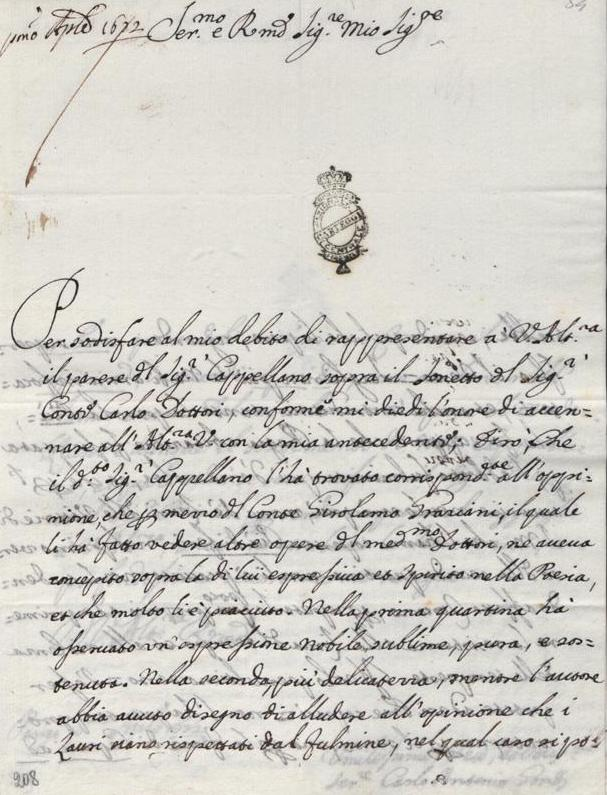
\includegraphics[width=0.37\textwidth]{24}
	\caption{An example of bleed-through}
	\centering
	\label{label:graph}
\end{figure}


In the study of this phenomenon we have come across many articles that deal with the subject and propose different removal techniques.
The various articles show that there are two types of removal methods 
%\cite{bleed1, bleed2}:
\begin{itemize}
  \item \textbf{Blind method}, one-sided information is used.
  \item \textbf{Non-blind method}, information is acquired from the front and back of the page.
\end{itemize}
Both methods have defects:
\begin{itemize}
  \item Blind methods are based on ink intensity, which can be problematic because there is a risk of eliminating "good" parts of the document, such as stamps and annotations.
  \item Regarding non-blind methods, we observed that the biggest problem concerns the perfect alignment between the recto and verso pages. Obviously, since these are online documents, the scanning may have distorted the actual alignment of the pages.
\end{itemize}
Most proposed methods are based on non-blind methods.

In order to clean the image, we experimented both types of methods.
In a first study we considered a non-blind method. We tried to create a filter that would remove dirt, comparing the two sides of the sheet, precisely subtracting them.
We then set ourselves the problem of alignment which we could not be able to solve.
Later on, we created a blind method which, through a Gaussian filter applied to the grayscale image, cleans the image from the bleed. We applied that method on 40 images and we created a database to learn a neural network that can automatically clean the image.

\section{\label{sec:level2}Cleaning Image}

\subsection{\label{sec:level2}Non blind method}
In order to remove bleed through we considered Recto and Verso of the image.
\begin{itemize}
  \item At first we create a mask consisting of a two-dimensional tensor composed initially by two recto and verso images.
  \item \textbf{The mask}: Recto and verso images are sequentially subtracted in order to obtain, in the first part of the two-dimensional tensor, a filter.
  \item Then we applied the mask to the image we wanted to correct.
\end{itemize}


\begin{lstlisting}[linewidth=\columnwidth,breaklines=true,language=python]
def maskElab(self,y):
        groups=[]
        groups2=[]
        groups3=[] 
        for j in range(2):
            group = layers.Lambda(lambda z: z[:,j,:,:])(y) 
            groups.append(group)          
        group2 = layers.Average()([groups[0], groups[1]])
        groups2.append(group2)         
        group2 = layers.Subtract()([groups[0], groups[1]])
        group2= layers.AveragePooling2D(pool_size=(1,1),strides=(1,1))(group2)  
        groups2.append(group2)       
        for gr in groups2:
            gr = layers.Lambda(lambda i : K.expand_dims(i, axis=1))(gr)
            groups3.append(gr)
        y= layers.concatenate(groups3,axis=1)
        y= layers.BatchNormalization()(y)  
        return y

\end{lstlisting}

\begin{figure*}%
\centering
\begin{subfigure}{.9\columnwidth}
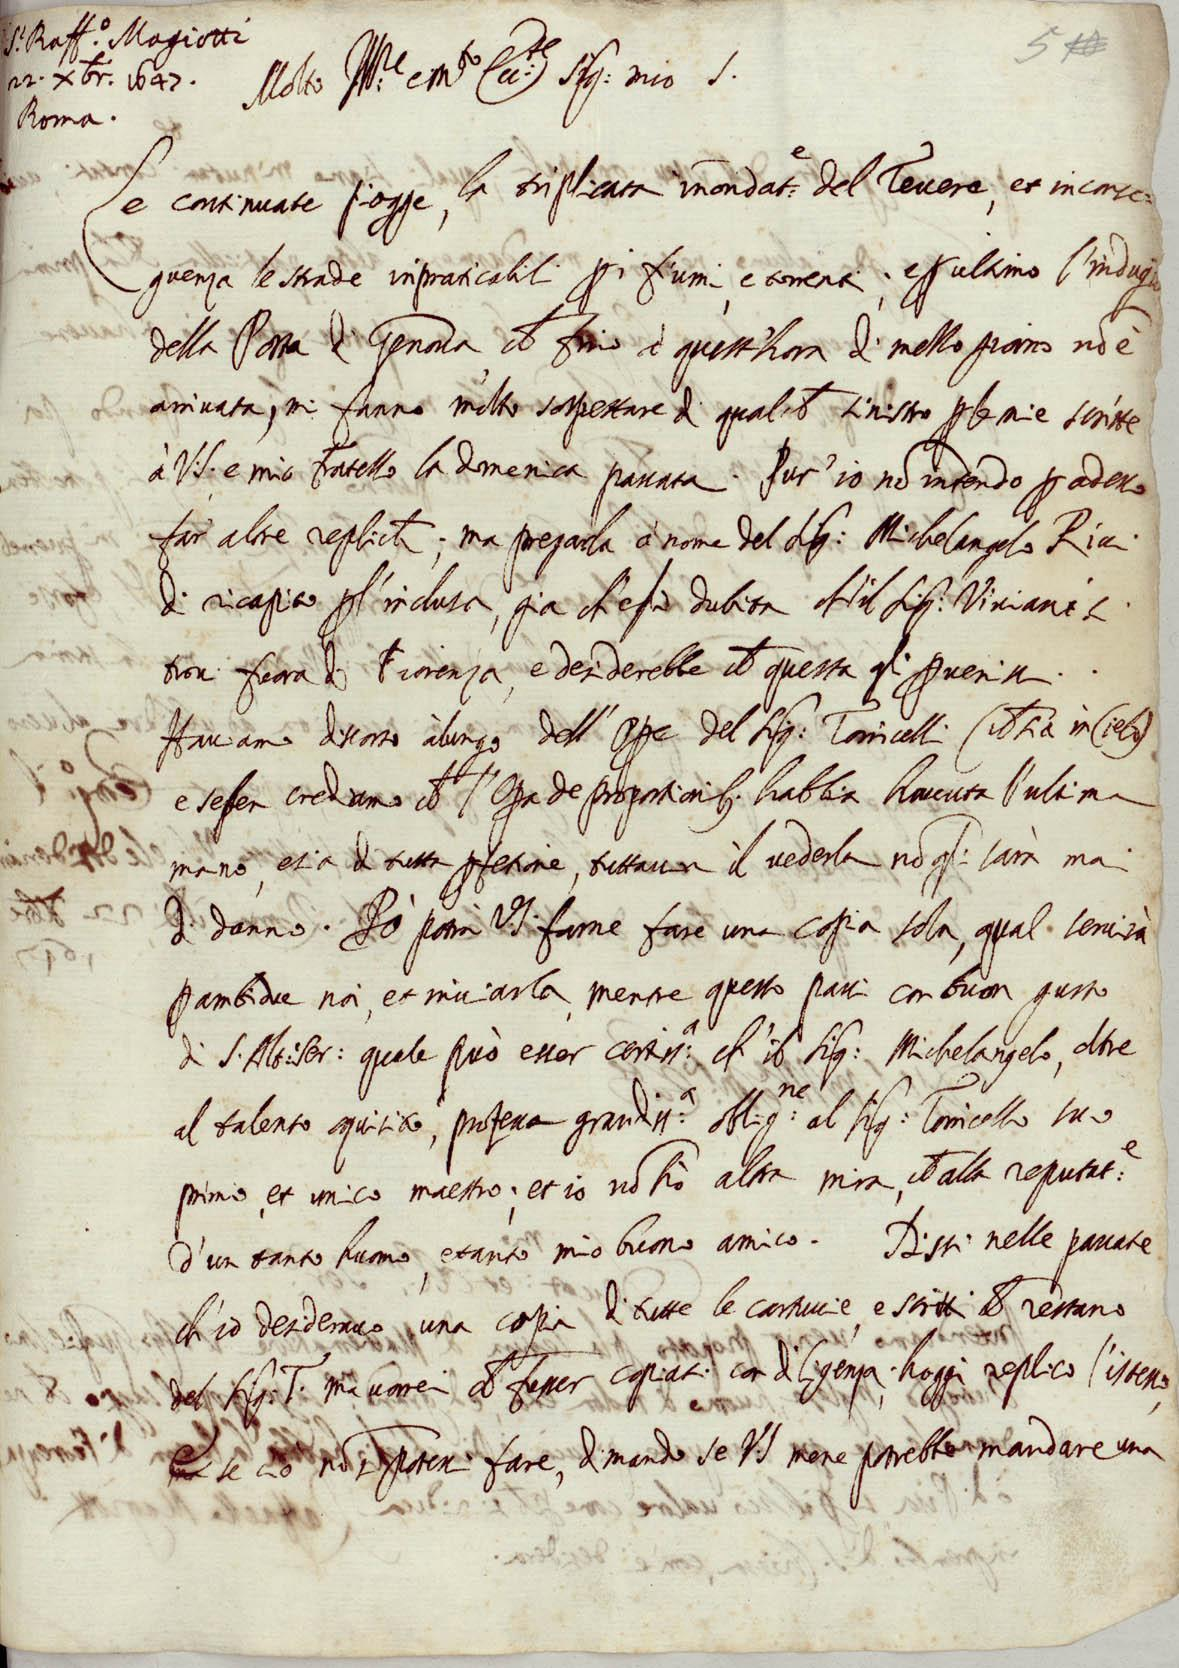
\includegraphics[width=\columnwidth]{gali2}%
\caption{Dirty image}%
\label{subfiga}%
\end{subfigure}\hfill%
\begin{subfigure}{.9\columnwidth}
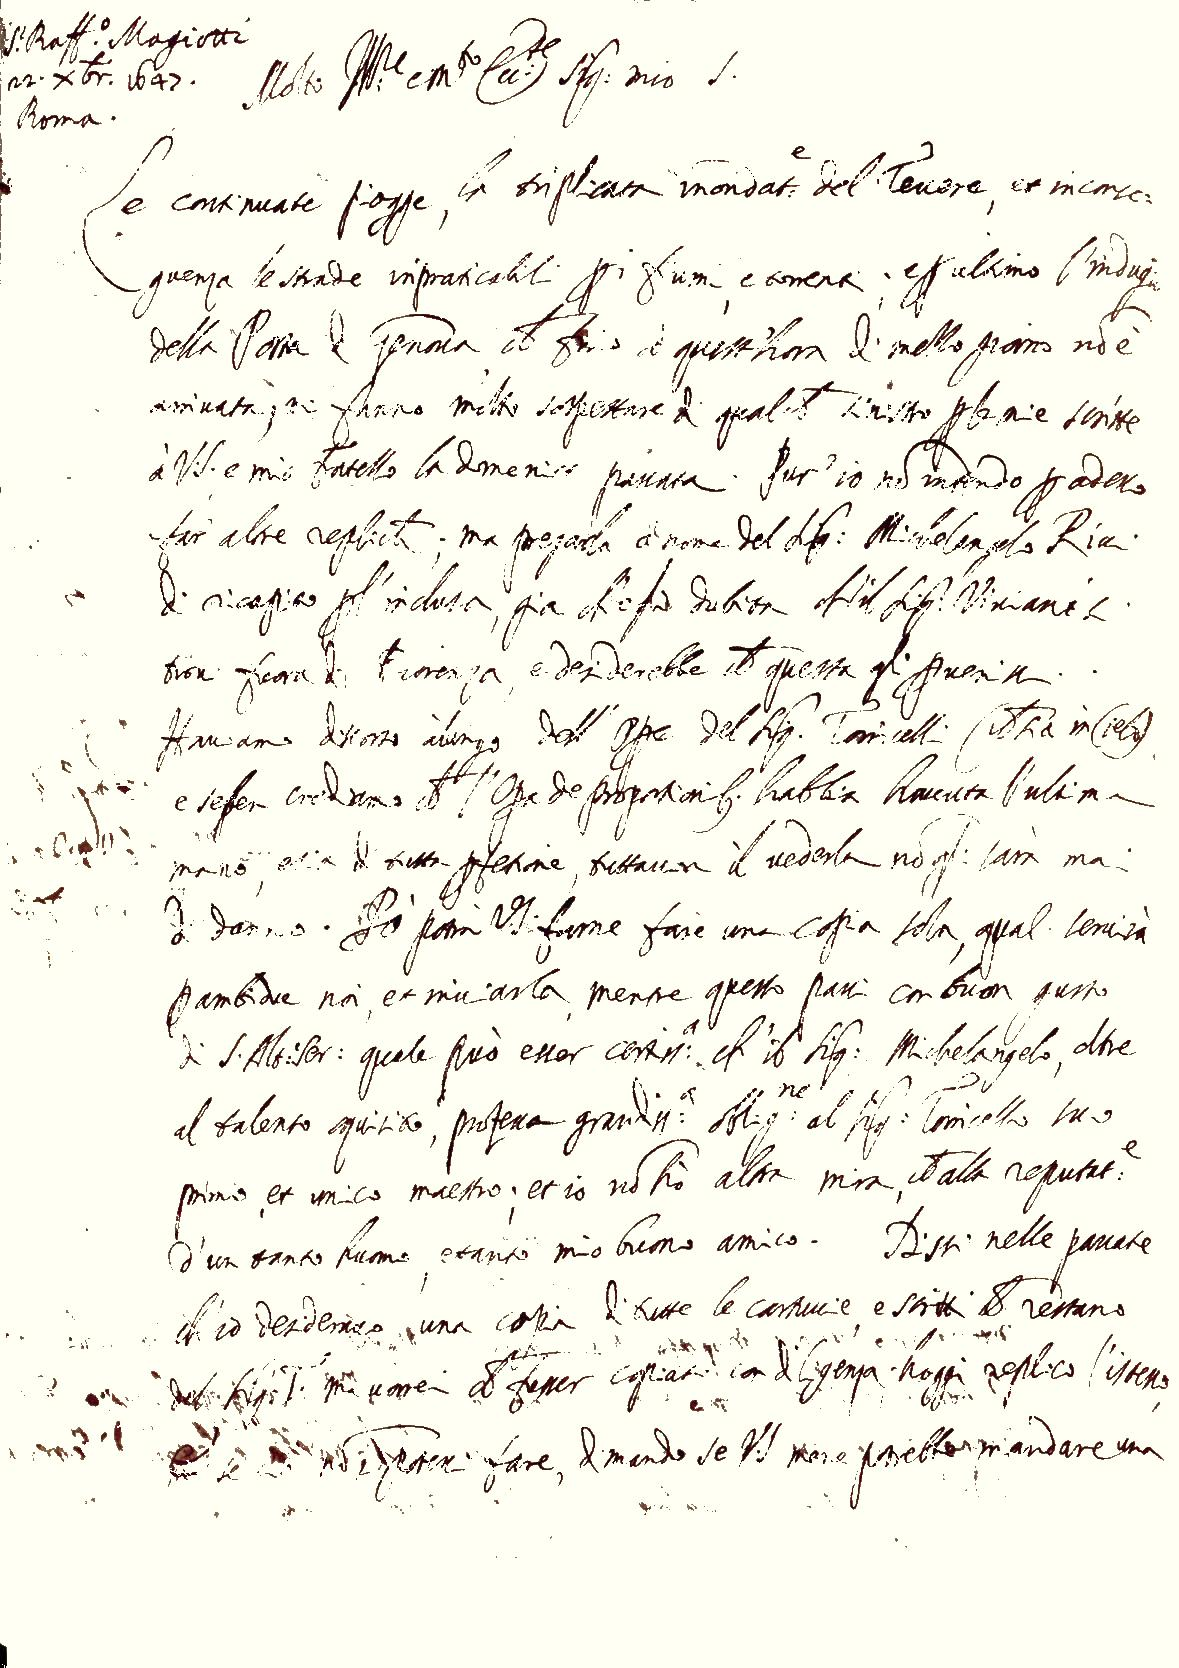
\includegraphics[width=\columnwidth]{gali2Pulito}%
\caption{Clean image}%
\label{subfigb}%
\end{subfigure}\hfill%
\caption{First Elaboration Project}
\label{figabc}
\end{figure*}

\subsection{\label{sec:level3}Alignment}
\subsubsection{Problems}
As we said before, the main problem of this approach is the alignment. We considered recto and verso and we have subtracted them, this operation mean that, for example considering recto as the image we want to clean, the recto's bleed should coincide with verso's written. 
This doesn't happen when we consider scanned document because, when a document is scanned or photographed, some amount of skew inevitably occurs in these documents.
%cite{bleed3}
 Even automatic image scanners are unable to perfectly align a document so that it is not tilted one way or the other.

\subsubsection{Proposed Solution}
We therefore thought about a solution to align the images extracting only the bleed from one of the two images (e.g. verso) and comparing it with the image cleaned by the bleed of the other direction (e.g. recto).
We realized two problems during the process:
\begin{itemize}
  \item We cannot bring out only the bleed because the contours of the "good" letters of the recto cannot be isolated from the bleed.
  \item Even if we could bring out only the bleed, we couldn't compare it with the verso image because it has the entire written and we would have an incomplete image. (see figure 3)
\end{itemize}

\begin{figure*}%
\centering
\begin{subfigure}{.9\columnwidth}
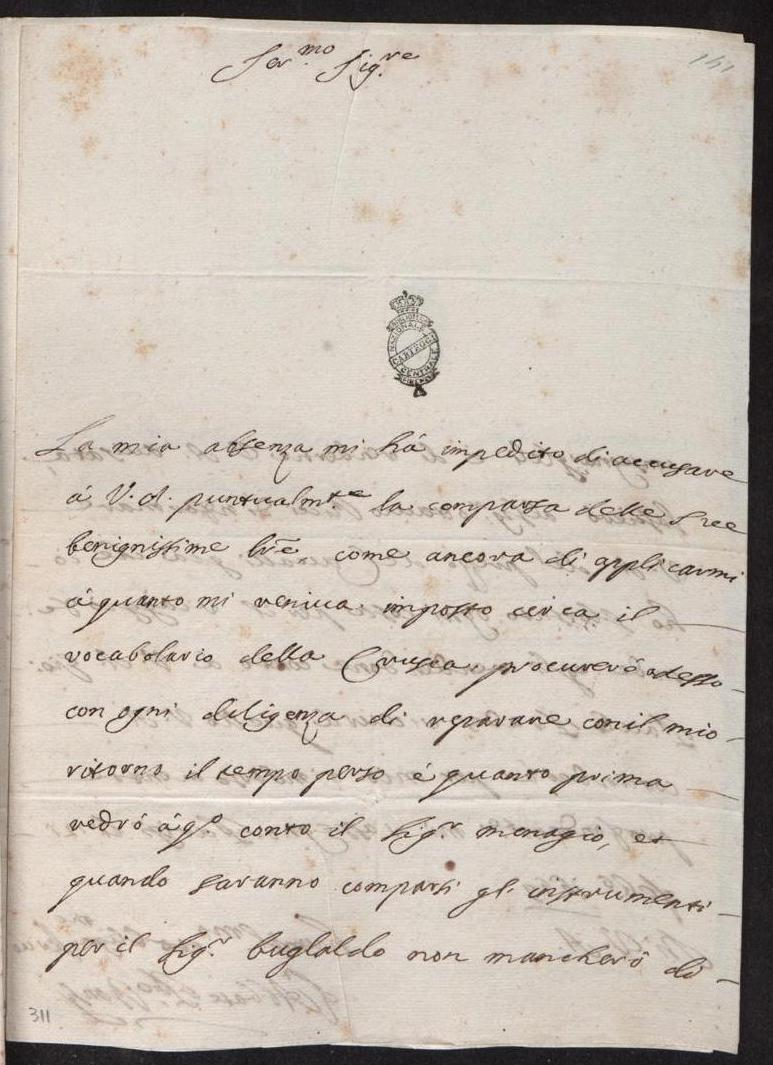
\includegraphics[width=\columnwidth]{45}%
\caption{Dirty image}%
\label{subfiga}%
\end{subfigure}\hfill%
\begin{subfigure}{.9\columnwidth}
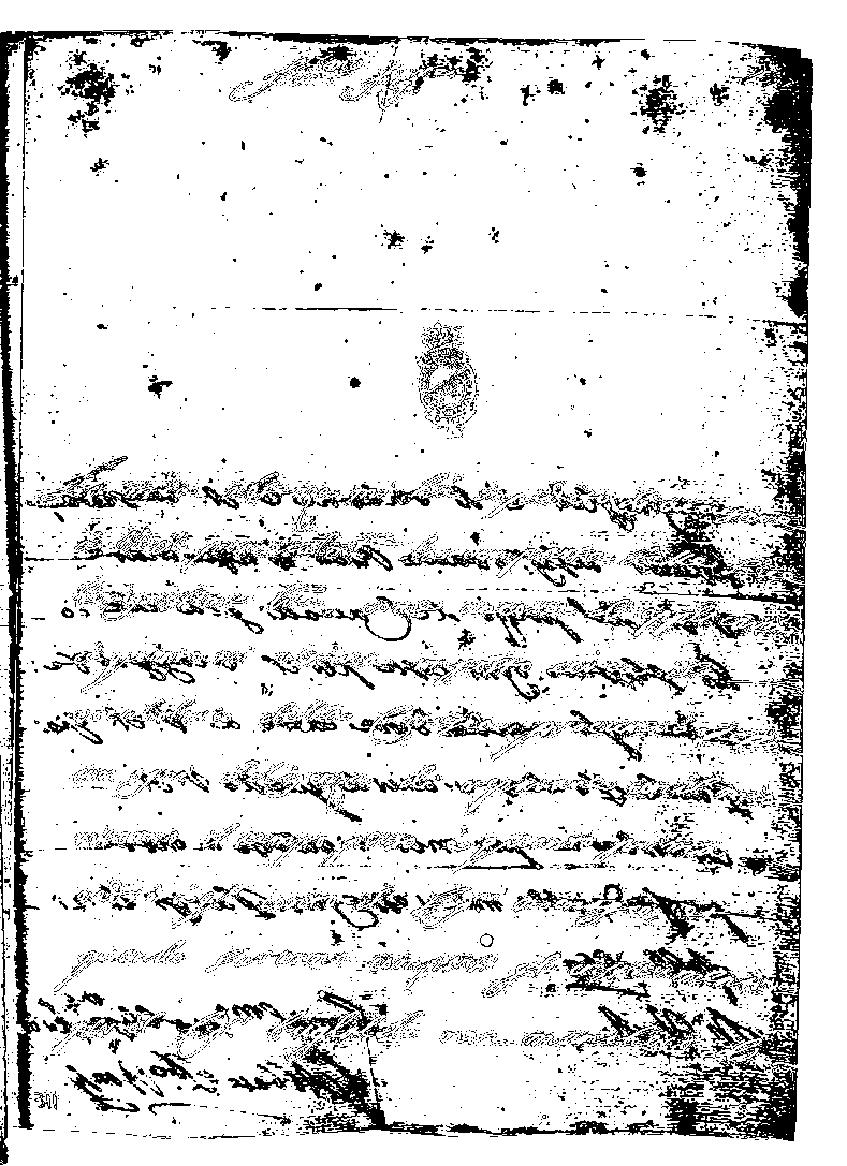
\includegraphics[width=\columnwidth]{bleedRetroSuFronte}%
\caption{Bleed retro on recto}%
\label{subfigb}%
\end{subfigure}\hfill%
\caption{Alignment problem}
\label{figabc}
\end{figure*}

\subsection{\label{sec:level4}Blind Method}
During the first part we were able to do the opposite of what we had proposed: considering an only image (recto or verso) we got the clean image through processing pixel to pixel.
By observing greyscale, we noticed that our document was composed of three levels:
\begin{itemize}
	\item Black: the written text we wanted to save.
	\item Grey: bleed and "good" written's boundaries.
	\item White: background.
\end{itemize}


\begin{table}[!ht]\footnotesize
	\centering
\begin{tabular}{l l l}
\toprule
\textbf{Image} & \textbf{Color} & \textbf{Threshold}\\
\midrule
Written front & black & 0-50 \\
Written verso & grey & 50-180 \\
Background & white & 180-255 \\
\bottomrule
\end{tabular}
\end{table}

\begin{table}[!ht]\footnotesize
	\centering
\begin{tabular}{l l}
\toprule
\textbf{Threshold} & \textbf{Normalization}\\
\midrule
0-50 & 0 \\
50-180 & 255 \\
180-255 & 255 \\
\bottomrule
\end{tabular}
\end{table}


So we have eliminated the bleed, bringing the gray levels corresponding to the background color.
We have eliminated pixel-to-pixel processing by assigning the task of bringing the gray pixels to 255 to a Gaussian function, with variance and mean variability depending on the image.
\begin{figure}[!ht]
	\centering
	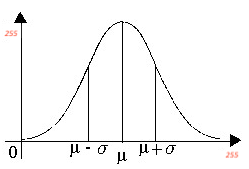
\includegraphics[width=0.5\textwidth]{gaussian}
	\caption{Gaussian Filter}
	\centering
	\label{Gaussian Filter}
\end{figure}


\begin{figure*}%
\centering
\begin{subfigure}{.9\columnwidth}
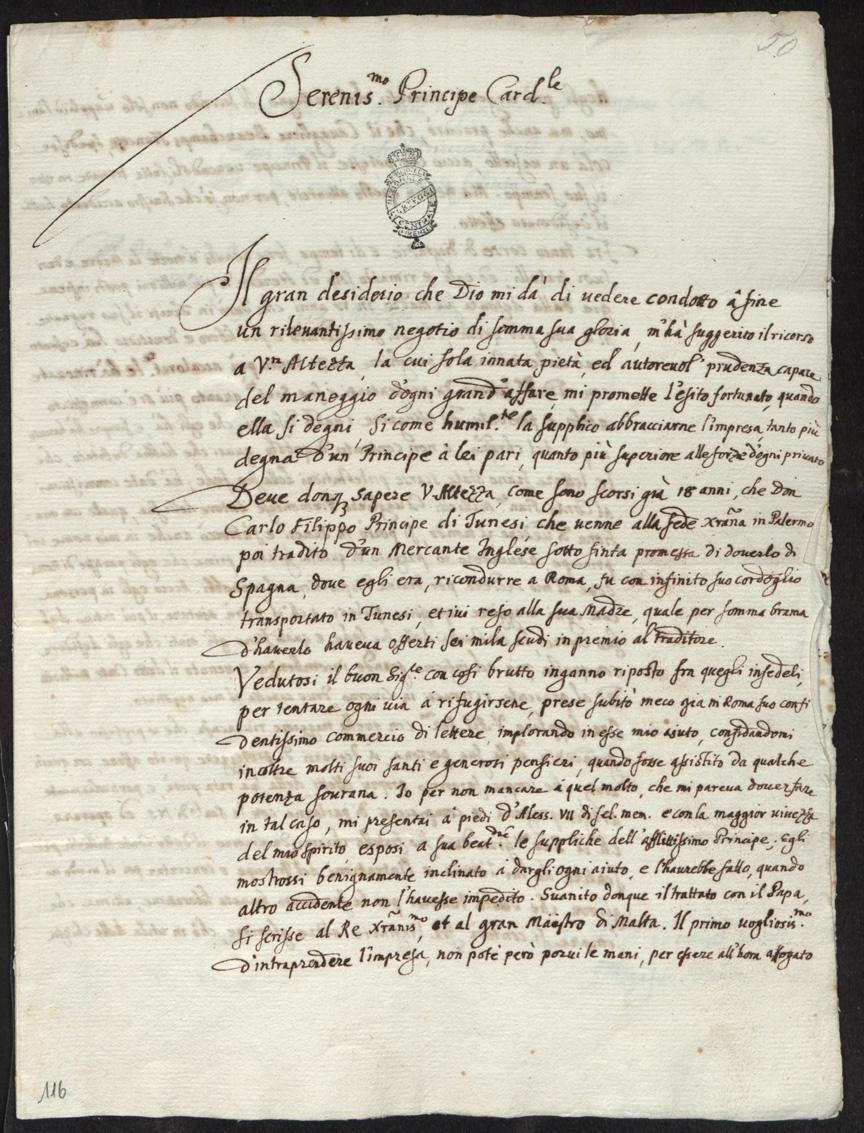
\includegraphics[width=\columnwidth]{35}%
\caption{Dirty image}%
\label{subfiga}%
\end{subfigure}\hfill%
\begin{subfigure}{.9\columnwidth}
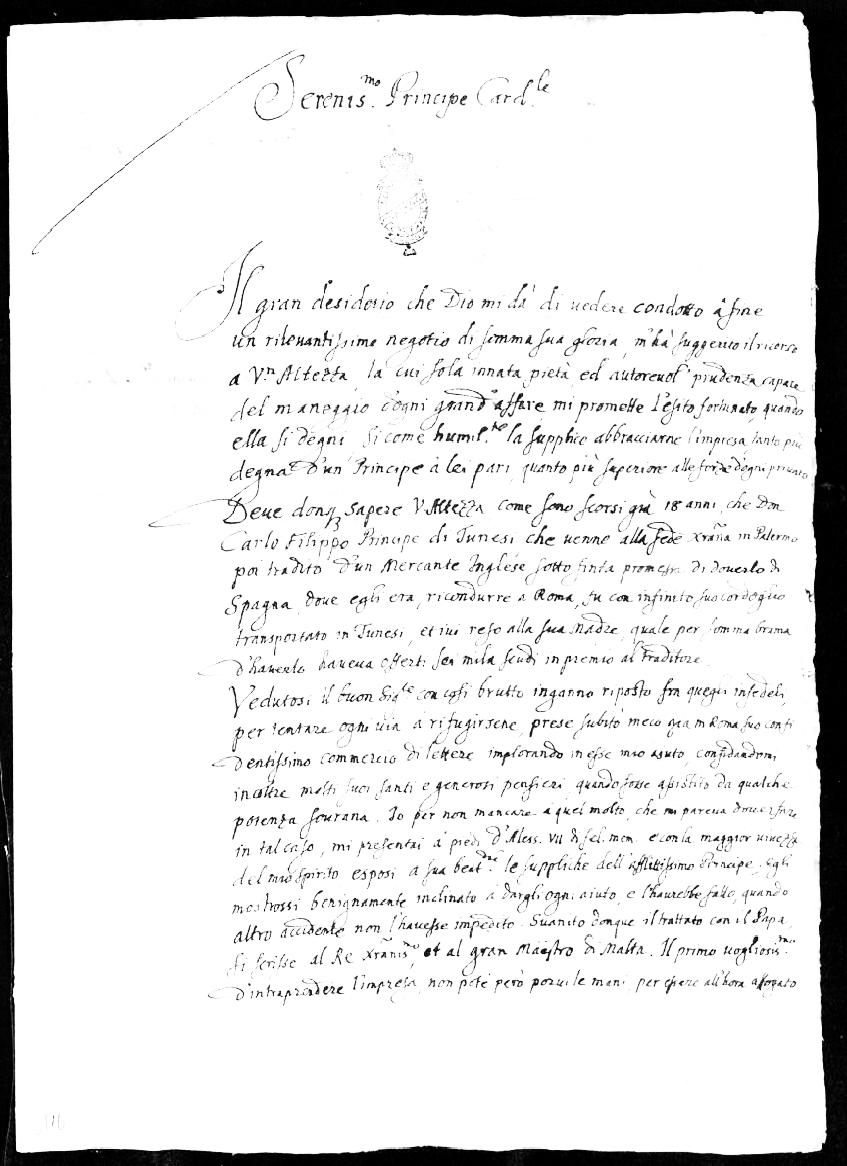
\includegraphics[width=\columnwidth]{35p}%
\caption{Clean image}%
\label{subfigb}%
\end{subfigure}\hfill%
\caption{Results}
\label{figabc}
\end{figure*}

\subsubsection{Results}
As shown in the image 5, we obtained an image cleaned up from the bleed in the background. During cleaning, the edges of the writing have eroded because, as already mentioned, they have the same gray tone as the bleed, but the result is to be considered satisfactory. We have also created a dataset consisting of 40 clean images obtained by appling the Gaussian filter methodology and we used them to instruct our neural network.

\section{\label{sec:level3}Neural Network}
To learn the network we used autoencoder.
An autoencoder is an unsupervised machine learning algorithm that takes an image as input and reconstructs it using fewer number of bits. The main difference between an autoencoder and a general purpose image compression algorithms is that in case of autoencoders, the compression is achieved by learning on a training set of data.

There are two parts to an autoencoder:

\begin{itemize}
  \item  \textbf{Encoder}: This is the part of the network that compresses the input into a fewer number of bits. The space represented by these fewer number of bits is called the 	“latent-space” and the point of maximum compression is called the bottleneck. These compressed bits that represent the original input are together called an “encoding” of the input.
  \item  \textbf{Decoder}: This is the part of the network that reconstructs the input image using the encoding of the image.
\end{itemize}

\begin{figure}[!ht]
	\centering
	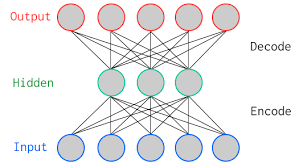
\includegraphics[width=0.8\columnwidth]{AutoEncoder}
	\caption{Autoencoder model}
	\centering
	\label{Autoencoder model}
\end{figure}

In the figure 6, we show a vanilla autoencoder (a 2-layer autoencoder with one hidden layer). The input and output layers have the same number of neurons. We feed five real values into the autoencoder which is compressed by the encoder into three real values at the bottleneck (middle layer). Using these three real values, the decoder tries to reconstruct the five real values which we had fed as an input to the network.


\subsection{First autoencoder} 
 Our first idea was to generate a classic autoencoder as shown in the figure. We applied our encoder to a dataset found in Internet, already divided into patches ($100 \times 100$). Two sets of images, train and test are provided. These images contain various styles of text, to which synthetic noise has been added to simulate messy and real-world artifacts. The training set includes the noise-free test (train-cleaned). An algorithm must be created to clean the images in the test set.
We used a convolutional autoencoder that use a "trick" consisting in replaceing fully connected layers by convolutional layers. These, along with pooling layers, convert the input from wide and thin (eg. $100 \times 100$ pixel with 3 channels RGB) to narrow and thick. This helps the network extract visual features from the images, and therefore obtain a much more accurate latent space representation. The reconstruction process uses upsampling and convolutions.
Convolutional autoencoders can be useful for reconstruction, for example, learn to remove noise from picture, or reconstruct missing parts.

\begin{lstlisting}[linewidth=\columnwidth,breaklines=true,language=python]
def build_autoencoder(input_size):
    input_img = Input(shape=(input_size,input_size,1), name= 'image_input')
    #encoder
    x = Conv2D(32,(3,3), activation='relu', padding='same', name='Conv1')(input_img)
 
    x = MaxPooling2D((2,2), padding='same', name='pool1')(x)
    x = Conv2D(64, (3,3), activation='relu', padding='same', name='Conv2')(x)

    x = MaxPooling2D((2,2), padding='same', name='pool2')(x) 
    x = Conv2D(64, (3,3), activation='relu', padding='same', name='Conv3')(x)

    x = MaxPooling2D((2,2), padding='same', name='pool3')(x) 
    x = Conv2D(64, (3,3), activation='relu', padding='same', name='Conv4')(x)
    #decoder
    x = MaxPooling2D((2,2), padding='same', name='pool4')(x) 
    x = Conv2D(64, (3,3), activation='relu', padding='same', name='Conv5')(x)
  
    x = UpSampling2D((2,2), name='upsample1')(x)
    x = Conv2D(64, (3,3), activation='relu', padding='same', name='Conv6')(x)

    x = UpSampling2D((2,2), name='upsample2')(x)
    x = Conv2D(64, (3,3), activation='relu', padding='same', name='Conv7')(x)

    x = UpSampling2D((2,2), name='upsample3')(x)
    x = Conv2D(32, (3,3), activation='relu', padding='same', name='Conv8')(x)

    x = UpSampling2D((2,2), name='upsample4')(x)
    x = Conv2D(1, (3,3), activation='sigmoid', padding='same', name='Conv9')(x)
    #model
    autoencoder = Model(inputs=input_img, outputs=x)
    autoencoder.compile(optimizer='adagrad', loss='binary_crossentropy')
    return autoencoder
\end{lstlisting}

\begin{figure}[!ht]
	\centering
	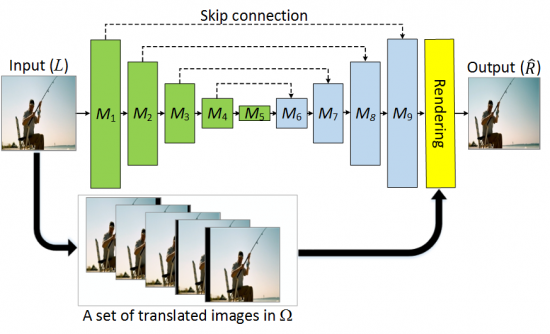
\includegraphics[width=0.8\columnwidth]{skip}
	\caption{Skip layers}
	\centering
	\label{Skip layers}
\end{figure}



\subsection{Second autoencoder} 
The results were not satisfactory because the network is composed of multiple layers of convolution operators, end-to-end learning mappings from corrupted images to the original ones. The convolutional layers act as the feature extractor which encode the primary components of image contents while eliminating the corruption. The de-convolutional layers then decode the image abstraction to recover the image content details.  We found a study that propose to add skip connections between corresponding convolutional and de-convolutional layers. 
%cite{skipLayers}
Our autoencoder recursively creates convolution levels (in the encoder) and deconvolution levels (in the decoder) and in the meantime it creates a link between the respective levels by adding them together.

\begin{lstlisting}[linewidth=\columnwidth,breaklines=true,language=python]
def recurrent_block(i,y):
    i -=1
    x = MaxPooling2D((2,2), padding='same')(y)
    x = Conv2D(64, (3,3), activation='relu', padding='same')(x)
    r = x 
    r = BatchNormalization()(r)
    if i < 0:
        x = MaxPooling2D((2,2), padding='same')(x)
        x = Conv2D(64, (3,3), activation='relu', padding='same')(x)          
    else:    
        x= recurrent_block(i,x)     
    x = UpSampling2D((2,2))(x)
    x = Conv2D(64, (3,3), activation='relu', padding='same')(x) 
    x= BatchNormalization()(x)
    x= Add()([x,r])
    return x 

\end{lstlisting}
Finally we set ourselves the problem of choosing the optimizer and we setted on gradient descent, that is one of the most popular algorithms to perform optimization and the most common way to optimize neural networks.
Gradient descent is a way to minimize an objective function J($\theta$) parameterized by a model's parameters $\theta$ $\in$ $\mathbb{R}^{d}$ by updating the parameters in the opposite direction of the gradient of the objective function \(\nabla_{\theta}J(\theta)\) with respect to the parameters. The learning rate determines the size of the steps we take to reach a (local) minimum. 
At first we used Adam, an adaptive learning rate optimization algorithm that’s been designed specifically for training deep neural networks.
We found many studies that demonstrates that to manage with RRN (recurrent networks) rmsprop algorithm was better than the other because these networks have a tendency to either vanish or explode as the energy is propagated through the function. And the effect has a cumulative nature, the more complex the function is, the worse the problem becomes.
Rmsprop can resolves the problem. It uses a moving average of squared gradients to normalize the gradient itself. That has an effect of balancing the step size, decrease the step for large gradient to avoid exploding, and increase the step for small gradient to avoid vanishing.
%cite{geoffreyhinton}
\begin{figure*}%
\centering
\begin{subfigure}{.9\columnwidth}
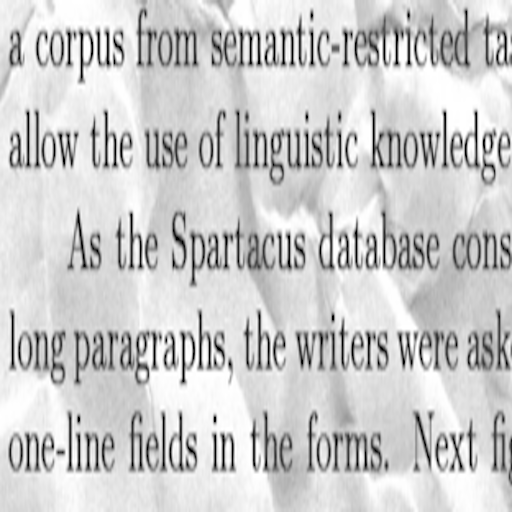
\includegraphics[width=\columnwidth]{original-k}%
\caption{Original}%
\label{subfiga}%
\end{subfigure}\hfill%
\begin{subfigure}{.9\columnwidth}
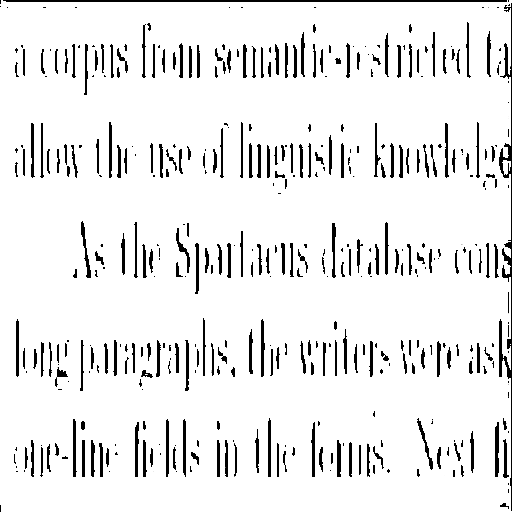
\includegraphics[width=\columnwidth]{autoEncoder-k}%
\caption{Result first Autoencoder}%
\label{subfigb}%
\end{subfigure}\hfill%
\caption{First Result}
\label{figabc}
\end{figure*}


\begin{figure*}%
\centering
\begin{subfigure}{.9\columnwidth}
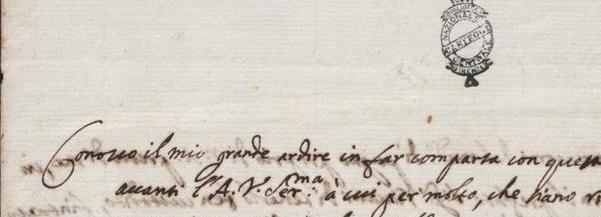
\includegraphics[width=\columnwidth]{second}%
\caption{Original}%
\label{subfiga}%
\end{subfigure}\hfill%
\begin{subfigure}{.9\columnwidth}
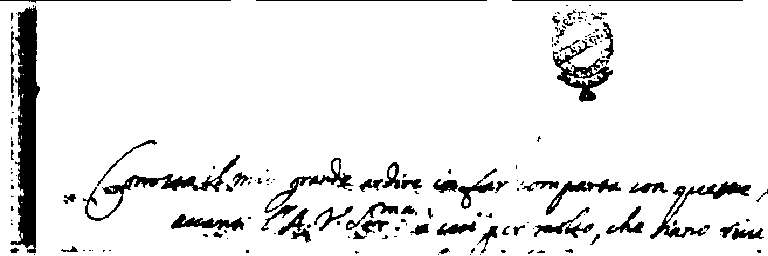
\includegraphics[width=\columnwidth]{secondAuto}%
\caption{Result second Autoencoder}%
\label{subfigb}%
\end{subfigure}\hfill%
\caption{Second Result}
\label{figabc}
\end{figure*}


\clearpage

%\bibliography{ArticoloBleedNotes}



\end{document}
%
% ****** End of file apssamp.tex ******